\documentclass{article}%
\usepackage[T1]{fontenc}%
\usepackage[utf8]{inputenc}%
\usepackage{lmodern}%
\usepackage{textcomp}%
\usepackage{lastpage}%
\usepackage{tikz}%
\usetikzlibrary{calc}%
%
\usetikzlibrary{arrows.meta}%
\usetikzlibrary{decorations.markings}%
%
\begin{document}%
\normalsize%
\normalsize%
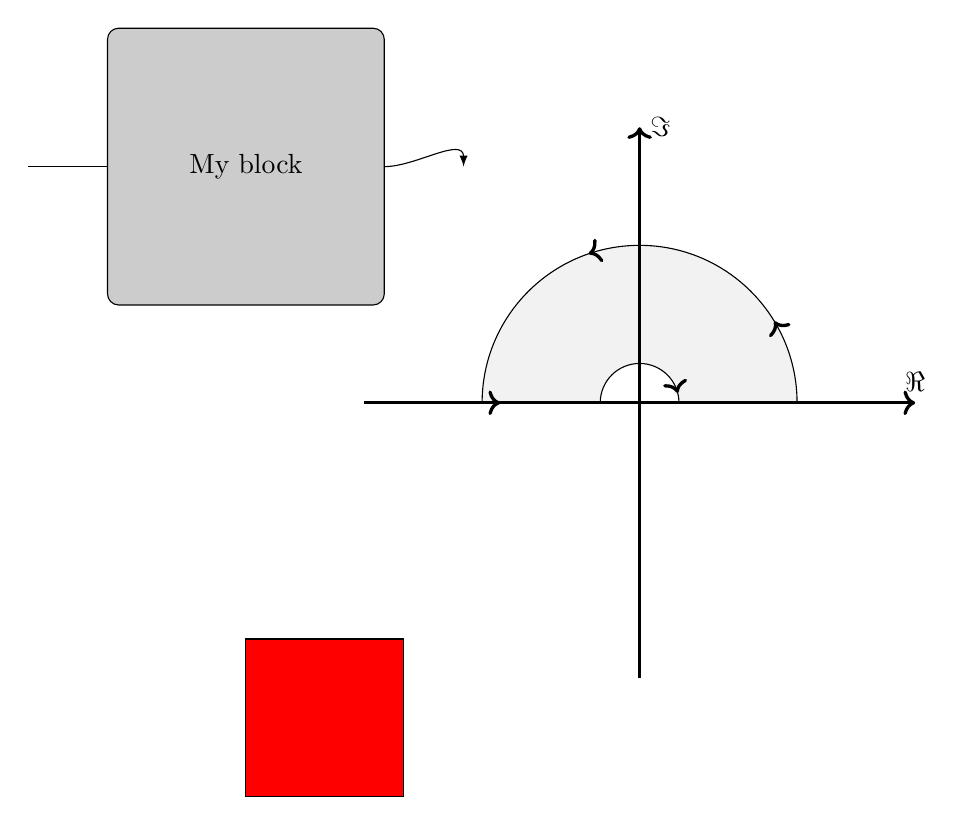
\begin{tikzpicture}%
\node[draw,rounded corners,align=center,minimum size=100pt,fill=black!20] (box) {My block};%
\draw[fill=red] (0.0,-6.0) rectangle (2.0,-8.0);%
\draw (box.west) -- ++(-1.0,0.0);%
\draw (box.east) edge[-latex,in=90,out=0] ++(1.0,0.0);%
\coordinate (orig) at (5.0,-3.0);%
\begin{scope}[decoration={markings,
mark=between positions 0.1 and 0.9 step 0.25 with {\arrow[very thick]{>}},}
,shift=(orig),scale=2]%
\draw[fill=gray!10,postaction=decorate] (0.0:1.0) arc (0.0:180.0:1.0) -- (180.0:0.25) arc (180.0:0.0:0.25) -- cycle;%
\end{scope}%
\draw[very thick,->] ($ (orig) + (-3.5,0.0) $) -- ($ (orig) + (3.5,0.0) $) node[above] {{$\Re$}};%
\draw[very thick,->] ($ (orig) + (0.0,-3.5) $) -- ($ (orig) + (0.0,3.5) $) node[right] {{$\Im$}};%
\end{tikzpicture}%
\end{document}